% 02.06.2016 12:00 CET last changed by a.holzinger
% General Template for LNCS and LNAI contributions based on llncs, adapted by ah
% Many thanks to the TRS team
% In case of using eps compile via 1) TeXify and then proceed with 2) dvi2pdf
%
\documentclass{llncs}
\usepackage{float}

\usepackage[dvips]{graphicx}
\usepackage[ruled,vlined]{algorithm2e}
\usepackage{amsfonts}
\usepackage{amssymb}
\usepackage{amsmath}
\usepackage{mathtools}

\providecommand{\abs}[1]{\lvert#1\rvert}
\providecommand{\norm}[1]{\lVert#1\rVert}

\usepackage{calc}
\usepackage{subfigure}

\usepackage{color}
\usepackage{soul}
\usepackage{comment}

\usepackage[font=small, labelfont=bf]{caption}

\newtheorem{prop}{Property}

\newenvironment{Bitemize}{\renewcommand\labelitemi{\textbullet}\begin{itemize}}{\end{itemize}}

\begin{document}

\title{The more the merrier - Federated learning from graph based recommendations}

% \author{Bernd Malle\inst{1}\inst{2}, Peter Kieseberg\inst{1}\inst{2}, Edgar Weippl\inst{2}, Andreas Holzinger\inst{1}}

%\institute{Holzinger Group HCI-KDD \\
%Institute for Medical Informatics, Statistics \& Documentation\\
%            Medical University Graz, Austria\\
%            \texttt{b.malle@hci-kdd.org}
%\and
%SBA Research gGmbH, Favoritenstraße 16, 1040 Wien \\
%			\texttt{PKieseberg@sba-research.org}
%}
	
\maketitle

% ==================================
%				ABSTRACT
% ==================================
\begin{abstract}
	
With Google's \textit{Federated Learning} \& Facebook's introduction of client-side NLP into their chat service, the era of client-side Machine Learning has finally begun. While interesting ML approaches beyond the realm of toy examples were hitherto confined to large data-centers and powerful GPU's, exponential trends in computing technology and the introduction of billions of smartphones bring sophisticated processing pipelines within reach of even hand-held devices. Such approaches hold several promises: 1. Without the need for powerful server infrastructures, even small companies could be scalable to millions of users easily and cost-efficiently; 2. Since data only used in the learning process never need to leave the client, personal information can be used free of privacy and data security concerns; 3. Since privacy is preserved automatically, the full range of personal information on the client device can be utilized for learning; and 4. without round-trips to the server, results like recommendations can be made available to users much faster, resulting in enhanced user experience. In this paper we propose an architecture for federated learning from personalized, graph based recommendations computed on client devices, collectively creating \& enhancing a global knowledge graph. In this network, individual users will 'train' their local recommender engines, while a server-based voting mechanism aggregates the developing client-side models, preventing over-fitting on highly subjective data from tarnishing the global model.

\medskip

\textbf{Keywords}: machine learning, federated learning, interactive learning, the local sphere, graph based recommendations, personalized ML models, distributed bagging


\end{abstract}

\renewcommand{\thesubfigure}{\thefigure.\arabic{subfigure}}
\makeatletter
\renewcommand{\p@subfigure}{}
\renewcommand{\@thesubfigure}{\thesubfigure:\hskip\subfiglabelskip}
\makeatother


% ==================================
%			INTRODCUTION
% ==================================
\section{Introduction and Motivation}
\label{sect:intro_motivation}

A 2006 paper \cite{leskovec2006recpatterns} examined recommender networks crystallizing from purchases based upon previously received product recommendations by employing an online shopping system observing purchases and recommendations of several product categories. Users of the platform were modeled as nodes in a graph with recommendations connecting them. This resulted in a collection of fragmented subgraphs representing series of so called \textit{recommendation cascades}. Their analysis revealed that about 95\% of all relevant recommendations originated from a subgraph with a diameter of only ~1.2, that is a node's immediate vicinity. Similar findings were also reported from the blogosphere \cite{leskovec2007blogpatterns}.

Observing a seemingly unrelated field of Software Development, the early 2010s have yielded new Web frameworks bringing the power of publish/subscribe systems within reach of even single developers. These mechanisms work by reconciling two potentially conflicting interests in a set-theoretic way: The set of all data-points a client wishes to receive are intersected with the set of all data-points a server is allowed to publish to specific individuals. This intersection is then pushed down to the client and constantly kept up to date, obviating the need for a client to permanently send new data / update requests. This leads to a certain sub-sample of global data permanently residing on the client device; in the case of a graph structure (social network, knowledge graph) this sub-sample would (at least) contain a node's immediate neighborhood.

Combining these two developments, we arrived at the definition of a \textit{local sphere} residing on a client device, representing a subset of the globally available information within a system. As for most recommendations those data points are seemingly the only ones relevant, we conjecture a new system architecture based on client-side, graph-based recommenders whose interaction with the user results in modifications of the local sphere, which by means of publish/subscribe are subsequently propagated throughout the system.

We therefore challenge the traditional notion of Machine Learning as happening on powerful, centralized servers and would like to replace them by a collective of mundane personal devices. Although this might seem futuristic, we see it as a logical solution especially to the problems of large-scale graph analysis \cite{leskovec2006samplinggraphs} as well as a continuation of a long-running trend towards employing commodity hardware for even the most demanding applications \cite{al2008scalable}.


\begin{figure}[H]
	\begin{center}
		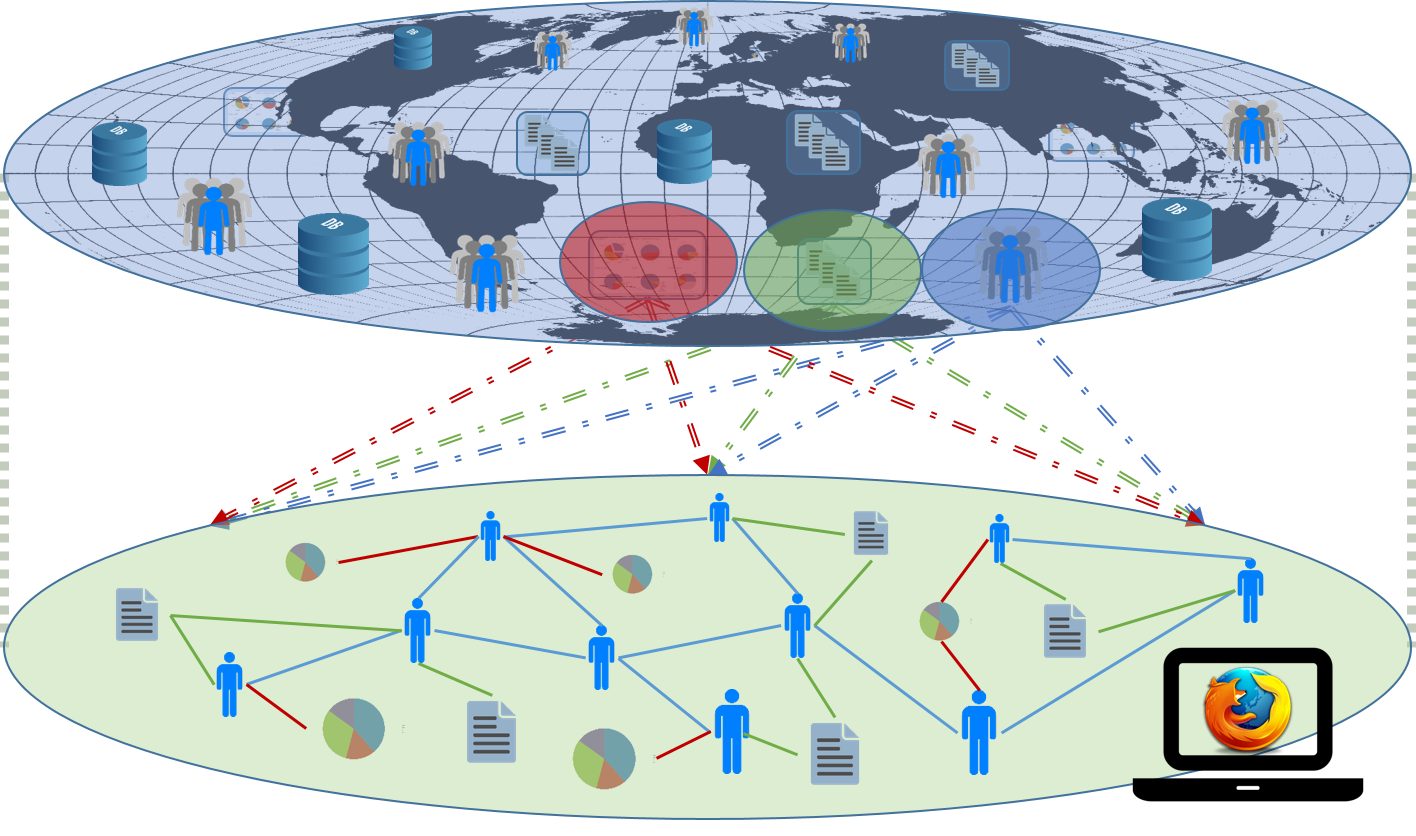
\includegraphics[width=0.8\textwidth]{figures/local_sphere}
		\caption{Publish-subscribe mechanism used by a client to constantly synchronize a subsample of a \textit{global database} to constitute what we term the \textit{local sphere}. Note that the local sphere is a superset of the user's data - it may contain items a user is not actually requesting, but might be significant for computing relevant recommendations.}
		\label{fig:local_sphere}
	\end{center}
\end{figure}



\section{Theoretical building blocks}
\label{sect:bg_related}

Aside from the engineering effort necessary to realize an architecture as we propose, we've identified 4 main theoretical aspects, or building-blocks, that could make it a target for novel scientific research, the confirmation and refinement of current theories, or even the formulation of new conjectures.

\subsection{Client-side Machine Learning}
\label{ssect:cs_ML}

... holds the promise of extreme scalability even for the smallest of startup companies. Because computations are mostly transferred to the client, organizations can limit their investment to the bare minimum of running any common Web-Site: Some servers transmitting snippets of client-side code as well as a sufficient database infrastructure. While there are still many challenges to overcome until client-side ML becomes ubiquitous, progress is already under way: Two teams \cite{mcmahan2016communication}, \cite{konevcny2016federatedlearning} report on a new distributed NN model that needs much less communication than synchronized SGD. As nodes in such a federated approach have but a tiny sub-sample of a traditional, global database, new algorithms are being devised for this setting \cite{konevcny2016federatedoptimization}. Because client-side computations might utilize personal information available only on a phone or tablet and model updates could inadvertently contain fragments of such information, secure server-side model aggregation has to be developed \cite{2017secureaggregation}.

%\cite{shi2012reciprocalrank}

\subsection{Privacy \& Security}
\label{ssect:privacy_security}

Privacy aware Machine Learning has been a hot topic for years \cite{wainwright2012paml} with its importance increasing dramatically due to ever intensifying limitations imposed by government regulations as well as public demand. One dramatic advantage of a distributed, client-side ML platform as we suggest it would be the isolation of privacy-endangering information within each user's personal device, rendering transfer of such information unnecessary, thereby effortlessly satisfying data protection regulations. On the other hand, learning on very small, subjective subsets of 'reality' could be seen as a profound distortion of data, and algorithms will have to be tested for suitability as well as stability in such scenarios \cite{malle2016right}.

\subsection{Interactive Machine Learning (iML)}
\label{ssect:iML}

Interactive ML algorithms adapt their models not just via feedback after their learning phase, but by continuously interacting with an outside \textit{oracle} (assumed to be omniscient), drawing positive / negative reinforcement from this interaction \cite{2016HolzingeriML}. Such systems are especially desirable in areas requiring highly-personalized predictions or decision support \cite{2016KiesebergDITL}; moreover human brains are known to be very good at approximating solutions and learning from a very small set of samples, thus enabling us to 'intuit' solutions that exact algorithms need (super)exponential time to resolve \cite{2016iMLExperiment}.

Since client-side recommenders in our proposed architecture would continuously compute \& provide users with individual recommendations which they can accept or reject, one could interpret this platform as a distributed system of interactive Machine Learning. As a consequence, one could transfer models learned by one user to new users of similar characteristic (however we obtain this information), thereby solving the notorious \textit{cold start} problem well known in the recommender community.


\subsection{Distributed Bagging}
\label{ssect:dist_bag}

Another intriguing aspect to our proposal comes from the field of ensemble learning, where Leo Breiman conceived the technique of \textit{Bagging} \cite{breiman1996bagging} in 1994. In Bagging (short for 'bootstrap aggregating') a global population is randomly sampled into several bags, so that each bag holds its own view of reality. Subsequently predictors are trained on these isolated sub-samples with the consequence of over-fitting on their respective, local data. Finally an aggregation mechanism fuses the local models back together, producing a much more stable global predictor.

Our local sphere approach might be seen as analogous to the idea of bagging, potentially distributed over billions of devices and with access to data not permissible in a central dataset. The overlapping of local spheres produces the same effect as sampling with replacement does for Bagging; the main difference of our strategy being the lack of randomness, since user-data are not actually 'sampled' from global knowledge. It remains to be seen if this difference presents a major drawback or actually an advantage.

\begin{figure}[H]
	\begin{center}
		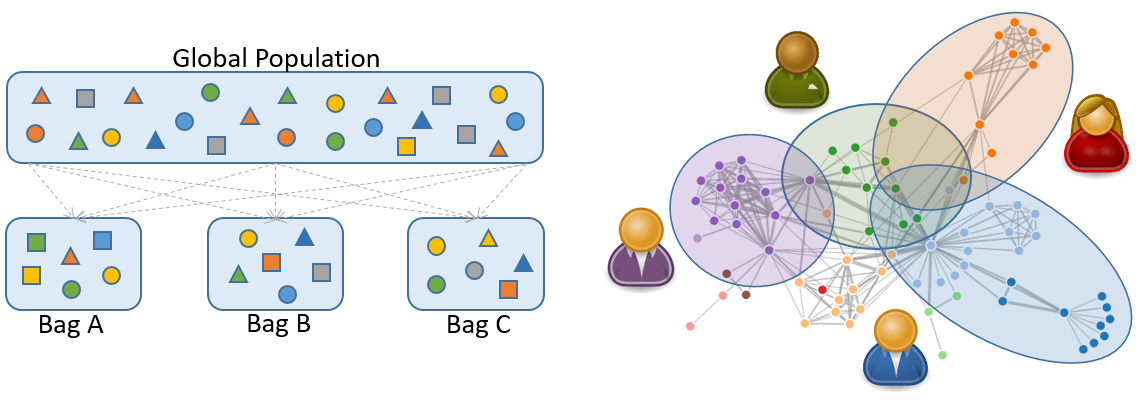
\includegraphics[width=1\textwidth]{figures/bagging_vs_local_sphere}
		\caption{Bagging vs. Spheres: To the left we depict the traditional bootstrap approach. To the right we see a global graph with user-defined \textit{local spheres}, which influence each other via their overlapping segments (albeit each residing on their respective client). The graph visualization was generated using D3.js \cite{zhu2013d3js}}
		\label{fig:bagging_vs_sphere}
	\end{center}
\end{figure}

% \vspace{-1cm}

\section{Proposed Workflow}
\label{sect:workflow}

In order to organize a perfect interplay of the components described above, we suggest the following sequence of interactions between the server (global sphere), client (local sphere), user (actually relevant data plus secure personal information) as well as the 'world' (all the information available on the Web or specialized online services):

\begin{enumerate}
	\item The client defines a subscription for all data which might interest the user.
	\item The server computes a local sphere by reconciling the client's request with it's own security / publication policy and pushes it down to the client.
	\item Once the local sphere is instantiated, the actually relevant user data are prepared \& visualized; the whole local sphere is instantiated within a client-side graph library in the background.
	\item Client-side recommender algorithms continuously check the local sphere that is not already part of the user data for possible new information and recommend them on occasion.
	\item Client-side \textit{gatherers} (e.g. web crawlers) utilize the users personal information accessible via her local device or social media account, scanning the web for suitable information items on every user interaction with the local sphere. Any extracted information items are again recommended to the user on a regular basis. A user's private data might even act as a personalized ontology and be combined with well-known knowledge extraction methods \cite{2003automaticKEfromWebDocuments}.
	\item The user interacts with her data via adding, connecting or re-arranging items. Each time new information is introduced into a local sphere it is synchronized to the server and - via it's overlapping segments with other local spheres - to those respective clients as well.
\end{enumerate}

As a consequence of this interactive workflow, it might even be possible to renounce the idea of a centrally curated global graph demanding tremendous computational power, energy as well as financial resources. Apart from occasional server-side sampling for reasons of security and general prudence, a global graph would emerge, be sustained and developed purely through the growth and / or modification of all the local spheres that fabricate it.


\section{Conclusion}
\label{sect:conclusion}

In this paper, we have welcomed the era of client-side machine learning and introduced the concept of the \textit{local sphere} as a logical building block for future collective (or federated) machine learning systems. We have derived the local sphere idea for graph-based recommendations from earlier works and defined the 4 theoretical building blocks of our proposed system, describing the advantage each of their underlying approaches contributes to the system. Finally, we presented a possible workflow architecture which would allow a global graph to exist entirely as an abstract, logical layer on top of a multitude of local sphere's interaction with one another and the rest of the world.

\newpage

\bibliographystyle{unsrt}
\bibliography{references}

\end{document}
